\section{Дашборд нагрузки поликлиники}

В данном разделе представлены основные визуализации, построенные на основе учебной базы данных поликлиники. Дашборд отражает распределение приёмов между врачами, динамику записей по датам, статусы приёмов и возрастную структуру пациентов.

\subsection{Распределение приёмов по специализациям врачей}

\begin{figure}[h!]
    \centering
    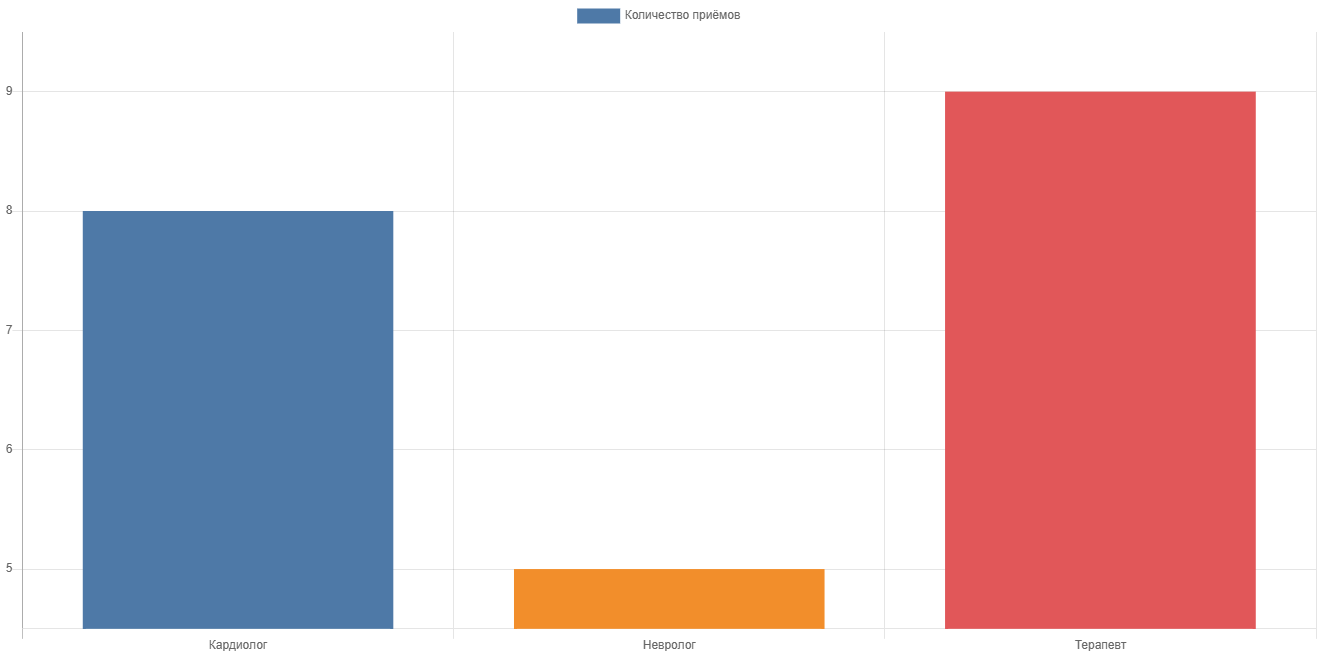
\includegraphics[width=0.75\textwidth]{charts/visits_by_specialty.png}
    \caption{Количество приёмов по специализациям врачей}
    \label{fig:visits_by_specialty}
\end{figure}

Столбчатая диаграмма на рис.~\ref{fig:visits_by_specialty} показывает, сколько приёмов приходится на каждого врача по специализации. Видно, что кардиолог обслуживает наибольшее число пациентов, тогда как невролог и терапевт имеют сопоставимую загрузку.

\subsection{Динамика числа приёмов по датам}

\begin{figure}[h!]
    \centering
    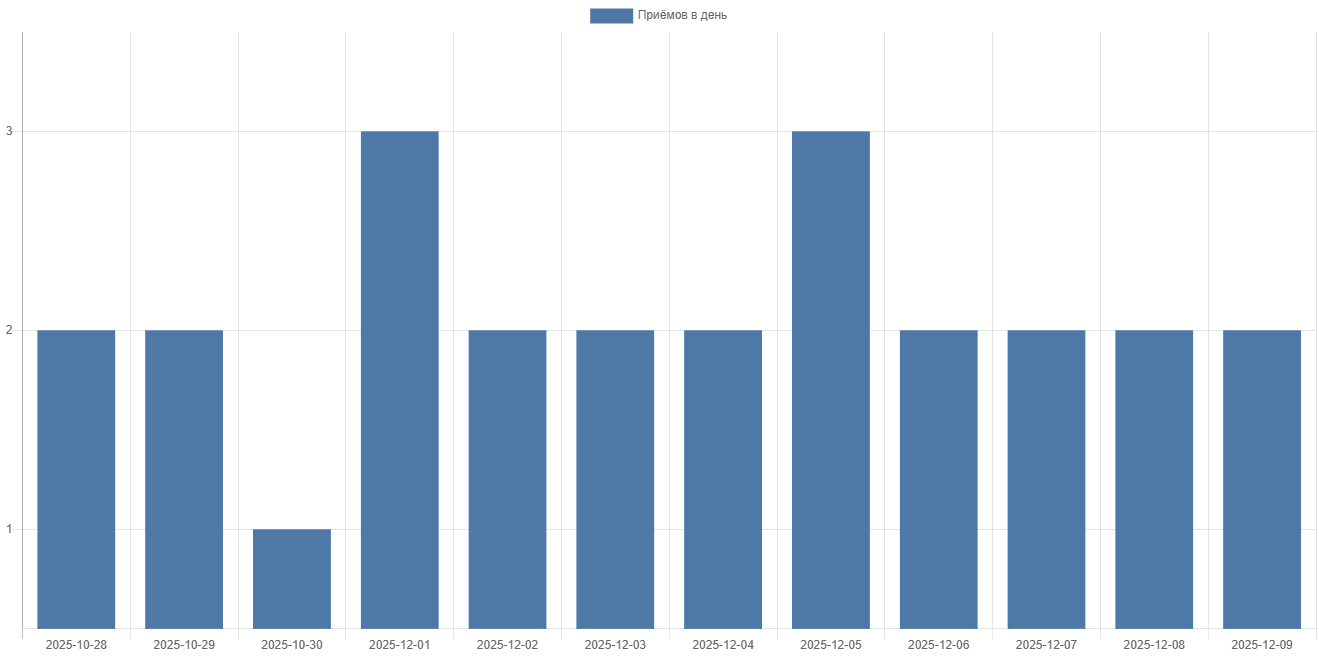
\includegraphics[width=0.75\textwidth]{charts/visits_by_date.png}
    \caption{Динамика количества приёмов по датам}
    \label{fig:visits_by_date}
\end{figure}

Столбчатая диаграмма на рис.~\ref{fig:visits_by_date} отражает, как меняется количество приёмов по календарным датам. Такая визуализация позволяет выделить дни с повышенной нагрузкой и оценить равномерность распределения записей во времени.

\subsection{Распределение приёмов по статусам}

\begin{figure}[h!]
    \centering
    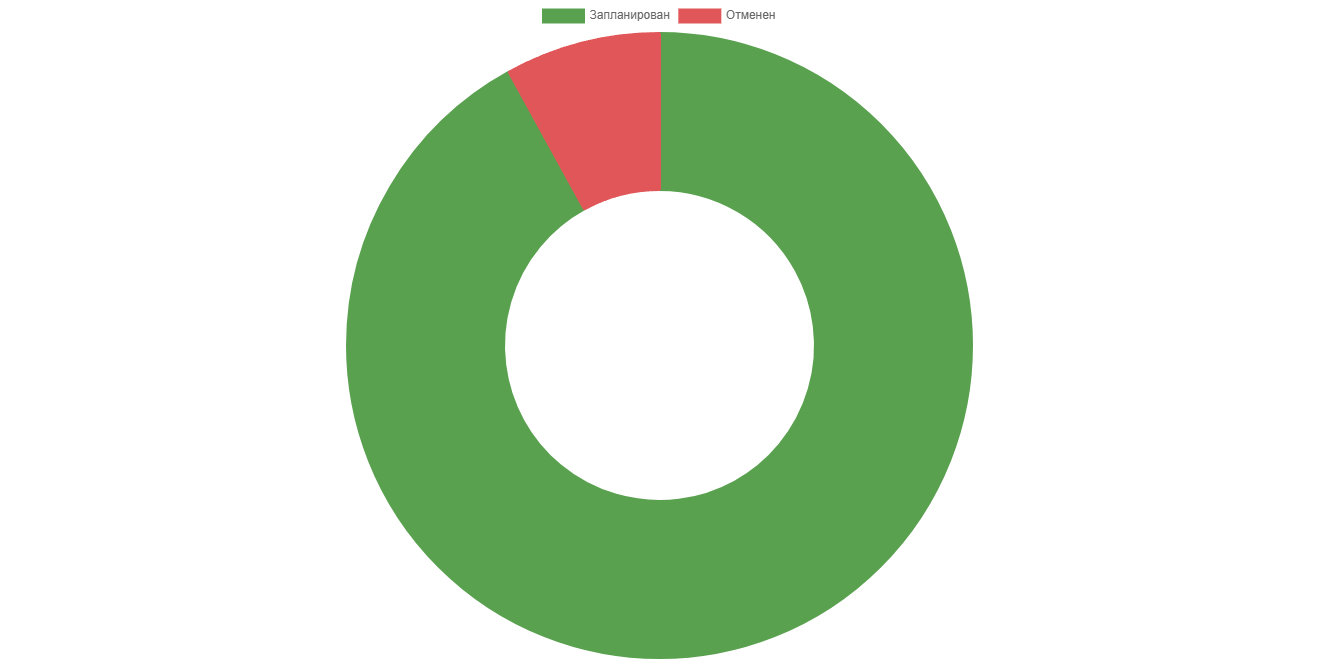
\includegraphics[width=0.6\textwidth]{charts/status_pie.png}
    \caption{Распределение приёмов по статусам}
    \label{fig:status_pie}
\end{figure}

Круговая диаграмма на рис.~\ref{fig:status_pie} демонстрирует долю приёмов в статусах <<Запланирован>> и <<Отменен>>. По ней можно оценить устойчивость записей и долю несостоявшихся приёмов относительно общего количества.

\subsection{Возрастная структура пациентов}

\begin{figure}[h!]
    \centering
    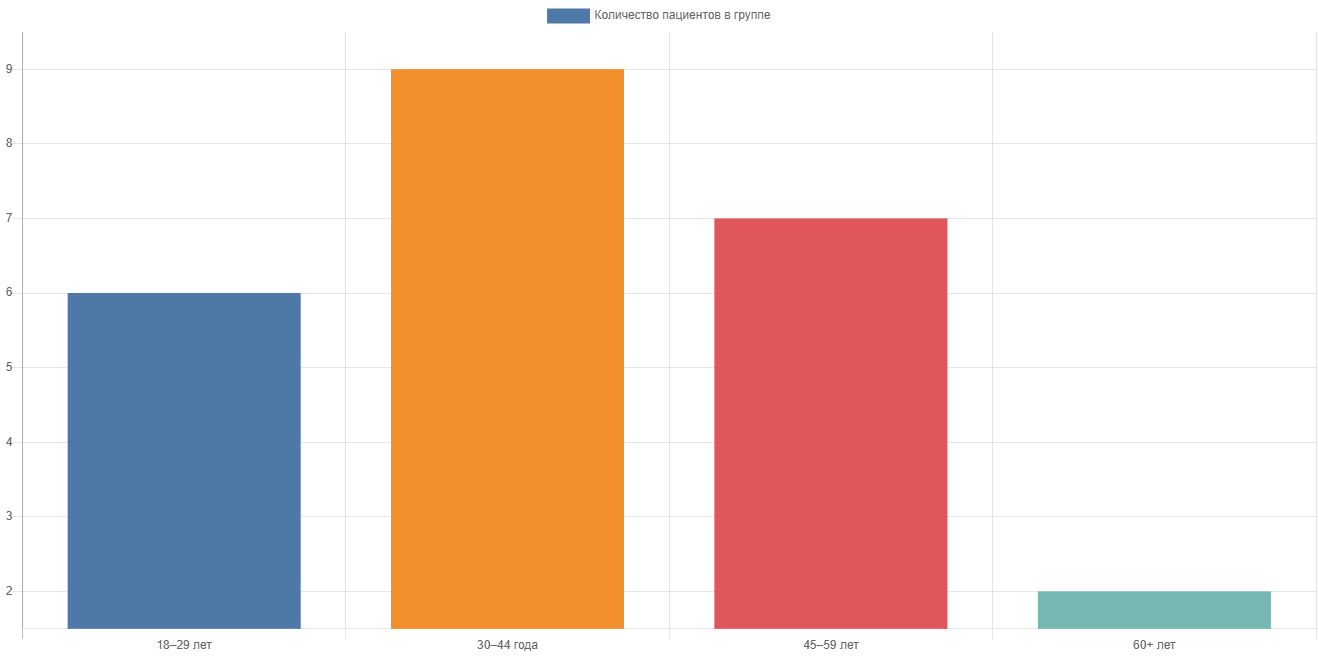
\includegraphics[width=0.75\textwidth]{charts/age_groups.png}
    \caption{Распределение пациентов по возрастным группам}
    \label{fig:age_groups}
\end{figure}

Столбчатая диаграмма на рис.~\ref{fig:age_groups} показывает распределение пациентов по основным возрастным группам. Такая информация важна для понимания целевой аудитории поликлиники и планирования нагрузки на врачей и оказываемые услуги.
